% arara: pdflatex
% arara: pdflatex
% arara: pdflatex

% options:
% thesis=B bachelor's thesis
% thesis=M master's thesis
% czech thesis in Czech language
% slovak thesis in Slovak language
% english thesis in English language
% hidelinks remove colour boxes around hyperlinks

\documentclass[thesis=B,czech]{FITthesis}[2019/12/23]

\usepackage[utf8]{inputenc} % LaTeX source encoded as UTF-8

\usepackage[T1]{fontenc}

% \usepackage{amsmath} %advanced maths
% \usepackage{amssymb} %additional math symbols

\usepackage{dirtree} %directory tree visualisation

% % list of acronyms
% \usepackage[acronym,nonumberlist,toc,numberedsection=autolabel]{glossaries}
% \iflanguage{czech}{\renewcommand*{\acronymname}{Seznam pou{\v z}it{\' y}ch zkratek}}{}
% \makeglossaries

\newcommand{\tg}{\mathop{\mathrm{tg}}} %cesky tangens
\newcommand{\cotg}{\mathop{\mathrm{cotg}}} %cesky cotangens

% % % % % % % % % % % % % % % % % % % % % % % % % % % % % % 
% ODTUD DAL VSE ZMENTE
% % % % % % % % % % % % % % % % % % % % % % % % % % % % % % 

\department{Katedra informační bezpečnosti (KIB)}

\title{Kubernetes klastr pro lámání hesel}

\authorGN{Tomáš} %(křestní) jméno (jména) autora

\authorFN{Klas} %příjmení autora

\authorWithDegrees{Tomáš Klas} %jméno autora včetně současných akademických titulů

\author{Tomáš Klas} %jméno autora bez akademických titulů

\supervisor{Ing. Jiří Buček, Ph.D. }

\acknowledgements{Doplňte, máte-li komu a za co děkovat. V~opačném případě úplně odstraňte tento příkaz.}

\abstractCS{Hlavní náplní práce je nakonfigurování klastru pro lámání hesel. Tento klastr je řízen pomocí technologie Kubernetes. Program využívá ke své správné funkcionalitě kontejnery. Tyto kontejnery jsou tzv. Docker kontejnery. Použité technologie jsou v práci detailně popsány a rozebrány. Dále se práce zabývá rešerží ukládání hesel v současných systémech a tím jak hesla vypadají. Na závěr na klastru bude proveden test různých metod pro lámání hesel. Tyto metody budou popsány a bude analyzováno, jak je klastr efektní a výkonný pro daný typ lámání. }

\abstractEN{The main goal of the thesis is to setup a cluster managed by kubernetes for password recovery. Next step is to describe used technologies as Docker, Ansible and Hashcat. Thesis contains description of how the passwords are stored and most known attacks to crack them. Successful deployment and password cracking leads to analyzing speed of the cluster and the particular cracking method. }

\placeForDeclarationOfAuthenticity{V~Praze}
\declarationOfAuthenticityOption{4} %volba Prohlášení (číslo 1-6)

\keywordsCS{Kubernetes, Ansible, klastr, Docker, distribuované lámání, hesla, hashcat, nasazení.}

\keywordsEN{Kubernetes, Ansible, cluster, Docker, distributed cracking, passwords, hashcat, deployment.}

% \website{http://site.example/thesis} %volitelná URL práce, objeví se v tiráži - úplně odstraňte, nemáte-li URL práce

\begin{document}

% \newacronym{CVUT}{{\v C}VUT}{{\v C}esk{\' e} vysok{\' e} u{\v c}en{\' i} technick{\' e} v Praze}
% \newacronym{FIT}{FIT}{Fakulta informa{\v c}n{\' i}ch technologi{\' i}}

% pomlcka --
% dlouha pomlcka ---
% vypustka \dots
% uvozovky \uv{text v uvozovkach} 
% cisla 
% barva \color{barevny text}
% prostredi pro vysvetlenia seznam \begin{description} listy maji sablony
% seznamy: enumerate, itemize, description
% poznamka pod carou \footnote{to co je pod carou}
% href{www.seznam.cz{seznamek}} = klikaci


\begin{introduction}
	%sem napište úvod Vaší práce
\end{introduction}

\chapter{Cíl práce}

Cílem práce je sestavit Kubernetes klastr, nasazen bude pomocí technologie Ansible a následně na něm bude spuštěn software na lámání hesel. Rychlost a výsledky lámání budou analyzovány s ohledem na délku hesla a použití daného druhu útoku. Budou popsány běžně používané útoky na hesla a způsob jejich ukládání na různých operačních systémech. Technologie, jež budou použity, budou popsány do hloubky nutné k porozumění daného řešení a následné možné replikace pro jiná řešení. 

\section{Kubernetes}

Jméno Kubernetes pochází z Řecka a znamená to kormidelník. Projekt zložili Joe Beda, Brendan Burns, a Craig McLuckie,ke kterým se rychle připojili inženýři z Googlu, jako Brian Grant a Tim Hockin. Software byl vydán v roce 2014.

Kubernetes je opensource technologie pro vytvoření a správu klastru. Pomáhá na tomto klastru plánovat spuštění kontejnerů na základě jeho stavu. Řídi automatickou aktualizaci kontejnerů a jejich opravu. Kontejnery sdružuje do podů, což je základní jednotka pro Kubernetes. Tyto pody škáluje na požadovaný stav.
Kubernetes také vyvažují zatížení a v případě pádu aplikace restartuje kontejner, aby znovu splnily požadavky.

\subsection{Stavební kameny Kubernetes}

Aby Kubernetes zajistili funkčnost klastru je zapotřebí rozdělit práci do několika komponent, které se starají o správný chod. Níže je znázorněno, z čeho se skládají. Dále se komponenty popíší a vysvětlí se na nich kompletní funkcionalita. 

\subsubsection{Master}



\subsubsection{Pod}



\subsubsection{Plánovač}



\subsubsection{Controller Manager}



\subsubsection{API server}



\subsubsection{Kubelet}



\subsubsection{Kube-Proxy}



\subsection{Kubernetes a tajemství}



\subsection{Aktualizace obraz}



\subsection{Sdílené datové prostory}



\subsection{Cloudový poskytovatelé}



\subsection{Flannel}



%\section{Ansible}

Ansible je automatizační nástroj pro konfiguraci systému, nasazení softwaru, aktualizac. Jeho nejsilnější stránka je nulové výpadky systému při aktualizaci balíčků, nebo automatické nastavovat dané zařízení. 

Jeho hlavními cíly jsou jednoduchost a nenáročnost. Kód by měl být čitelný i pro lidi, kteří nejsou obeznámeni s programem. Je schopen pokrýt různě velké prostředí od malých podniků až po velice obsáhlou infrastrukturu. 

Ansible se připojí na vzdálený počítač pomocí OpenSSH pomocí uživatele, který je současně přihlášen. Na spravovaném počítači není trřeba žádný agent. Je možnost nakonfigurovat Ansible, aby pro připojení nepoužíval OpenSSH, ale i kerberos nebo LDAP. 

\subsection{Komponenty}

\subsubsection{Control node}

Jakýkoliv počítač s nainstalovaným Ansible a pythonem, může spouštět příkazy nebo tzv. playbooky. Tento počítač se nazývá control node. Takových můžeme mít klidně více, ne však počítače, které mají nainstalovaný operační systém Windows. 

\subsubsection{Managed node}

Je jakékoliv síťové zařízení. Managed nodes můžeme také nayývat jako hosts. Tyto zařízení nemusejí mít nainstalovaný Ansible, ale musejí mít nainstalovaný python. Ansible může být nakofigurován, aby používal specifikovanou verzi pythonu, pokud není specifikována, spustí se na hostu jeho defaultní.

\subsubsection{Iventory}

Je seznam všech nastavovaných zařízení. Často se nazývá hostfile. v tomto souboru nastavujeme skupiny zařízení, jejich IP adresy a další specifikace, například jaký python má daný host použít. 

\subsubsection{Modules}

Jsou to jednotlivé části kódu, které bude Ansible spouštět. Každý modul má speciální použití. Vše od správy uživatelů ( user ) přes nastavení systému ( systemd ) až k instalovaní balíčků ( apt, yum ). Můžeme spustit jeden modul v tasku, nebo více v playbooku. Pro přehlednost neuvádím všechnz možné moduly, jelikož je jich přes tři tisíce. 

\subsubsection{Tasks}

Jsou jednotky, které se museji provést. Nejčasteji specifikované v deployment souboru. 

\subsubsection{Playbooks}

Je seřazený seznam tasků, které se musí vykonat. Ničemu neuškodí pokud se plazbook spustí znovu, protože Asnible skontroluje stav daného tasku. Playbooky jsou psané podle konvenci YAMLu. 


\section{Docker}

Docker je otevřená platforma pro vývoj, dodání a spouštění aplikací. Umožnuje oddělení aplikací od infrastruktury, tedy můžeme dodávat software rychleji a bez problémů, které se váží k různorodosti prostředí, ve kterém aplikace běží. Svou fylozofií jsou velice podobné virtualním počítačům. Rozdíly mezi těmito různými pohledy na věc budou rozebrány dále v textu. 

Docker zprostředkovává platformu pro zabalení aplikace i se všemi jejímy závislostmi. Izoluje danou aplikaci od ostatních běžících procesů na daném počítači a zajišťuje tak její bezpečí. Docker kontejner je velice nenáročný na hardware, můžeme jich tedy na daném počítači spustit velice mnoho.  

Fylosofie kontejnerů je taková, že každý kontejner je odpovědný pouze za jednu danou část aplikace. Pro příklad máme naší webovou aplikaci. Budeme tedy mít alespoň tři docker kontejnery. Jeden na kterém poběží NGINX a bude zprostředkovávat naší aplikaci uživatelům. Další bude mít naší aplikaci a ve třetím poběží databáze. 

Konterjnery fungují tedy jako malé počítače, mají izolované veškeré svoje systémové zdroje ( paměť, procesy, internetové rozhraní ). Díky tomuto mohou být rychle a jednoduše přidány, nebo odebrány.  


\subsection{Konterjner vs. virtuální počítač}

Virtualizace je odpověď na problém různorodých prostředí mezi vývojáři a zákazníky. Problém ,který virtualizace a kontejnerizace především řeší je různorodost prostředí mezi zákazníkem a dodavatelem softwaru. Při jeho předávání dochází ke změně prostředí, jsou nainstalované jiné verze závislostí a operačního systému a aplikace se může chovat neočekávaně. 

Podíváme se jak se tyto dvě technologie liší a proč se svět žene právě směrem kontejnerizace, když zde již je řešení.

Virtuální počítač je regulérní stroj, který běží na daném hostovi. Tento stroj má svůj kernel, svůj operační systém a ke zdrojům přistupuje přes tzv. hypervizor např.: QEMU, nebo VirtualBox. Hypervizor zprostředkovává přístup virtuálního stroje k systémovým zdrojům. 

Pro to, aby na hostovi, nebo-li na systému, který má nainstalovaný hypervizor mohlo běžet více virtuálních strojů stačí jedna jeho instance. Nevýhoda tohoto řešení je taková, že se mnoho zdrojů duplikuje. Řekněme, že na hostitelském systému poběží tři aplikace. Každá taková aplikace bude izolovaná od ostatních pomocí virtuálního stroje. Dejme tomu, že to bude databáze, webový server a stroj pro vzdáleného uživatele. Níže uvidíme nákres tohoto řešení. 

% https://www.docker.com/resources/what-container
\begin{figure}[!h]
	\centering
	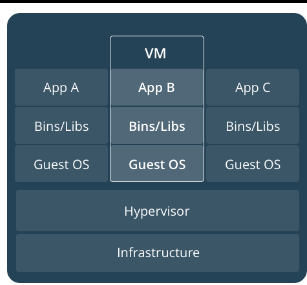
\includegraphics[width=0.73\textwidth, angle=0]{docker-VM.png}
	\caption[Docker VM]{Oddělení aplikací za pomoci hypervizoru a virtuálních strojů.}
	\label{fig:docker-vm}
\end{figure}

To samé, jako je na obrázku výše se pokusíme realizovat pomocí Dockeru a kontejnerů. Kontejnery, jelikož využívají overlayFS jsou schopny poskytnout jádro operačního systému kontejneru bez zbytečné kopie a využívají copy-on-write funkcionality. Níže uvidíme jak za pomoci jmenných prostorů, kontrolních skupin a overlayFS je tento přístup úspornější a rychlejší než virtualizace. 


\begin{figure}[!h]
	\centering
	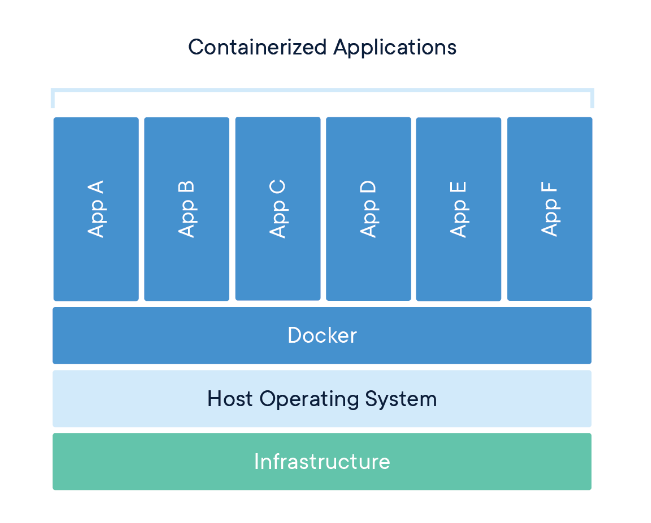
\includegraphics[width=0.8\textwidth, angle=0]{docker-docker.png}
	\caption[Docker kontejnery]{Oddělení aplikací za pomoci Dockeru}
	\label{fig:docker-docker}
\end{figure}

Místo, které jsme na hostitelském systému ušetřili však není jediná výhoda. Na tomto příkladu se však rozdíly mezi těmito technologiemi vysvětlují nejlépe. Dalšími výhodami je rychlost spuštění kontejneru a virtuálního stroje. Při spuštění se pouze připojí obraz OS, vytvoří se izolované procesy a popřípadě se omezí i zdroje, které má kontejner využívat. Nehledě na to, že pokud kontejner nemá omezení nebo limit využitých zdrojů alokuje si je dynamicky oproti virtuálnímu počítači, který si pro sebe naalokuje danou paměť při spuštění.  


\subsection{Stavební kameny Dockeru}

Jak je již uvedeno v předešlé kapitole, Docker využívá vychytávky linuxového kernelu pro svojí funkcionalitu. Díky tomuto perfektně funguje na počítačích, kde běží OS založený na Linuxu. V následujících sekcích budou tyto technologie blíže popsány a bude vysvětlena jejich důležitost. 

\begin{figure}[!h]
	\centering
	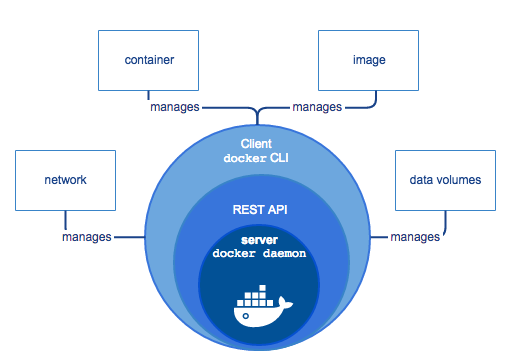
\includegraphics[width=0.8\textwidth, angle=0]{docker-architecture.png}
	\caption[Docker architektura]{Docker a jeho komponenty.}
	\label{fig:docker-architecture}
\end{figure}

%TODO Jak jsou na tom jiné OS

\subsubsection{Jmenné prostory}

Jmenné prostory zastřešují veškeré zdroje systému tak, že každý proces spuštěn v daném prostoru může používat pouze prostředky, které se váží k tomuto prostoru. Každému procesu se to jeví tak, že má svoje vlastní globální prostředky, které mohou vidět i ostatní procesy z jmenného prostoru, ale ne z jiného. V tabulce \ref{tab:Jmenne prostory} je možné videt, jaké jmenné prostory lze v Linuxu nalézt.

% parametry pro table: h! = nejblize
% p{5cm} na zalomovani bunky
\begin{table}[h!]
  \begin{center}
	\caption{Linuxové jmenné prostory}
    \label{tab:Jmenne prostory}
    \begin{tabular}{|l|l|} 
    	  \hline
      \textbf{Jméno} & \textbf{Popis} \\
      \hline

	  Cgroup  &  Cgroup root adresář\\
	  IPC     &  Systém pro komunikaci procesů, POSIX fronty\\
	  Network &  Síťové rozhraní, protocoly, porty, etc\\
      Mount   &  Připojená zařízení\\
      PID     &  ID procesů\\
      User    &  Uživatelská ID a ID skupin\\
      UTS     &  Hostname a NIS doménu\\   
      
      \hline
    \end{tabular}
  \end{center}
\end{table}

Při spuštění kontejneru dojde k vytvoření procesu na hostitelském systému. Procesy dostanou od systému nějaké PID a chovají se jako normální procesy. Pokud se však přihlásíme do kontejneru (command: docker exec -it name bash) a podíváme se na procesy běžící v daném kontejneru uvidíme, že procesy mají jiná PID a určitě mají i PID=1. Toto nám umožňují jmenné prostory.

Každý kontejner může mít svůj vlastní souborový systém a svoje síťové rozhraní. Vše co můžeme oddělit mezi hostitelem a kontejnery je uvedeno v tabulce výše. 

\subsubsection{Kontrolní skupina}

Je to vlastnost Linuxového kernelu. Jejich hlavní funkcí je limitovat zdroje. V Dockeru se používají protože dovolují sdílet prostředky mezi hostitelským systémem a dalšímy kontejnery. 

Často dochází k záměně pojmů mezi kontrolními skupinami a jmennými prostory. Znovu to tedy shrňme. Kontrolní skupinz, nebo-li cgroups omezují co můžeme použít a jemenné prostorz nebo-li namespaces omezují co jsme schopni vidět v systému. 

\subsubsection{Docker daemon}

Docker daemon nebo-li dockerd poslouchá dotazy na docker API a spravuje objekty jakou jsou docker obrazy, kontejnery, síť a úložiště. Komunikuje ale i s dalšími daemony, aby byl schopen řídit službu Docker.

\subsubsection{Docker klient}

Je to primární cesta, jak komunikovat s Dockerem. Když použijeme příkazy, jako jsou "docker run", klient odešle příkazy daemono zmíněného výše. 

\subsubsection{Docker registr}

Docker registr je úložiště pro naše Docker obrazy. Bez předchozího nastavení hledá dockerd obrazy, které chceme spustit ve veřejném Docker registru. Obrazy však mohou být dostupné i lokálně, nebo na nějaké jiné službě, např.: gitlab container registry. 

Do styku s registrem přícházíme hlavně ve chvílích, kdy provádíme příkazý docker pull, docker push a docker run. Tyto příkazy vždy potřebují znát obraz, který bude spouštěn jako základní vrstva pro nový kontejner, nebo bude stáhnut na lokání počítač, či nasdílen do registru.

\subsubsection{Obrazy}

Můžeme si to představit jako šablonu, na které je spuštěn kontejner. Obraz může být složen z vícero obrazů, nebo z nich vycházet. 

Pro vytvoření obrazu je třeba soubor Dockerfile. Tento soubor obsahuje jednoduché kroky, které je třeba vykonat pro vytvoření konkrétního obrazu. Např.: jaké použijeme a zveřejníme porty, jaké balíčky chceme ve vytvořeném obrazu mít atd. 

Každý příkaz v Dockerfilu vytvoří na locálním počítači tzv. vrstvu, kterou při úpravě Dockerfilu mění nebo předělává pouze pokud byla změněna. 

%TODO picture of docker architecture

\subsection{Systémová kontejnery}

Docker kontejnery nejsou však jediné, které se v produkčním prostředí používají. Patří do tzv. aplikačních kontejnerů. Jejich účel je zpravidla spouštět pouze jeden proces. K takovýmto kontejnerům můžeme ještě přidat kontejnerz Rocket. Hlavním rozdílem je to, že rtk nemá na systému spuštěného daemona jako má např. Docker. Při spuštění se tedy pod běžícím spustí další. 

Dále tady máme systémové kontejnery. Ty jsou používané jako klasické OS. Na jednom silném stroji může běžet několik takových kontejnerů a ty mohou uživateli poskytovat oddělené prostředí od celého serveru a nabídnout mu izolovaný prostor od ostattních pomocí výše zmíněných technologií. Tuto možnost zastřešuje projekt LXC později LXD.

%TODO add image of the lxc list




\chapter{Hesla}

Hesla můžeme vidět všude a ne jen v informatice. 
Pokud se podíváme zpět do historie např. do doby velkého Caesara a jeho šifry, ke které je třeba znát číslo, o které se posouvají znaky ve zprávě. 
Jak tedy můžeme vidět, hesla neslouži pouze k naší autentizaci vůči nějaké službě či serveru. 
Můžeme je také použít k podepsání citlivých dokumentů jako je třeba příloha e-mailu. 
Následně pak nemůžeme popřít jeho poslání. Tomuto se říká elektronický podpis. 

Hesla však mají nejednu nevýhodu. Útočník může s naším, nebo i bez našeho vědění odhalit naše heslo a tím nám narušit naše soukromí. Hesla mohou také být v systémech, které používáme uložena nepatřičným způsobem, jako je například čistý text bez použití žádných ochranných prostředků. 

Hesla též mohou ze systému uniknout. V tomto případě, pokud byla hesla uložena neptřičným způsobem nemusí se potencionální útočník nějak přemáhat, aby uživatele kompromitoval. Proto se zaměříme na to jak mohou a jak skutečně jsou uložena. 

\section{Windows}
% https://cs.wikipedia.org/wiki/NTLM
Windows se chovají jinak v doméně a jinak mimo ní. Pokud je počítač v doméně je preferován autentizační protokol kerberos. V doméně je nastaven jeden nebo více autentikačních serverů přes které se uživatel ověřuje. V současných Windows Server edicích je implementován Kerberos verze 5. Kerberos v základní nastavenim operuje na portu 88 a k šifrování používá symetrickou šifru. 
Pokud počítač není nastaven aby se autentikoval pomocí protokolu Kerberos používají Windows šifrování NTLM. Tento protokol autentizace není oficiálně dokumentován, byl však popsán v projektu Samba. Současná nejnvoější verze je označena NTLMv2.

\subsection{Popis protokolu}

Protokol se řídí sekvencí výzva-odpověď, která vyžaduje, aby mezi klientem a serverem  byly vyměněny celkem tři zprávy (three-way-handshake):

\begin{enumerate}
	\item Klient odešle zprávu obsahující informace o klientem podporovaných nebo požadovaných funkcích (velikosti kryptovacích klíčů, požadavek na vzájemnou autentizaci atd.)
	\item Server odpoví zprávou obsahující podobné informace o serverem podporovaných nebo požadovaných funkcích (čímž klient dokáže vybrat vhodné autentizační parametry) a - nejdůležitější část - náhodnou výzvu (8 bytů, tzv kryptografická sůl).
	\item Klient pak použije výzvu ze zprávy, uživatelské jméno a heslo k vypočtení odpovědi. Volba výpočetní metody je závislá na autentizačních parametrech dohodnutých předešlou zprávou, nicméně obecně lze říci, že aplikuje hašovací funkce MD4 nebo MD5 a šifrování DES.
\end{enumerate}

%https://wiki.wizard32.net/xwiki/bin/view/Penetration%20Testing_Red%20Teaming/NTLM%20Relay%20Attack/
\begin{figure}[!ht]
	\centering
 	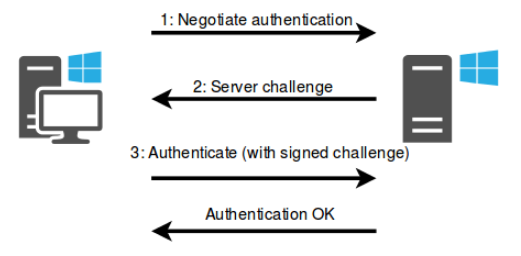
\includegraphics[width=0.8\textwidth, angle=0]{hesla-windows.png}
 	\caption[Hesla windows]{NTLM protokol pro autentizaci.}\label{fig:windows}
\end{figure}

\section{Linux}

Linux jakožto systém, který se skládá pouze ze souborů má též hesla uložena v jednom souboru \path{/etc/shadow}. Hesla v linuxu bývala dříve uložena společně v \path{/etc/passwd}. Kvůli bezpešnosti se však oddělila a v souboru byl otisk nahrazen pismenem x. Hesla jsou uložena pomocí zvolené hašovací funkce. V tabulce níže uvidíme podporované funkce.


% parametry pro table: h! = nejblize
% p{5cm} na zalomovani bunky
\begin{table}[!ht]
  \begin{center}
	\caption{Hašovací funkce}
    \label{tab:Hash funkce}
    \begin{tabular}{|l|l|} 
    	  \hline
      \textbf{ID} & \textbf{Funkce} \\
      \hline

	  1  &  MD5\\
	  2a &  Blowfish\\
	  5  &  SHA-256\\
      6  &  SHA-512\\

      \hline
    \end{tabular}
  \end{center}
\end{table}

%TODO better shadow structure

\section{Hešovací funkce}

% https://link.springer.com/content/pdf/10.1007%2F978-3-540-25937-4_24.pdf
% https://knihy.nic.cz/files/edice/Kryptografie_okolo_nas.pdf

Hešovací funkce je kryptografická funkce, která argumentu o prakticky libovolné délce přiřazuje tzv. heš H, což je číselná hodnota o pevně stanovené délce (typicky o délce 256 až 512 bitů). 
Od hešovací funkce se vyžadují dvě specifické vlastnosti:

\begin{itemize}
	\item \textbf{Jednosměrnost}, což znamená, že určení hodnoty heše je pro zadaný vzor výpočetně snadné, avšak určení hodnoty vzoru ze znalosti jeho heše je prakticky nemožné.
	\item \textbf{Bezkoliznost}, což znamená, že je prakticky nemožné nalézt nějakou dvojici různých vzorů takovou, aby jejich heše byly stejné. V této souvislosti je zapotřebí si uvědomit, že počet číselných posloupností libovolné délky (tj. počet vzorů) je vždy větší než počet posloupností jediné možné délky. Z toho pak plyne, že mnoho vzorů musí mít stejný heš a vznikají tak kolize. Požaduje se však, aby nalezení kolize bylo prakticky nemožné.
\end{itemize}

\begin{figure}[!ht]
	\centering
 	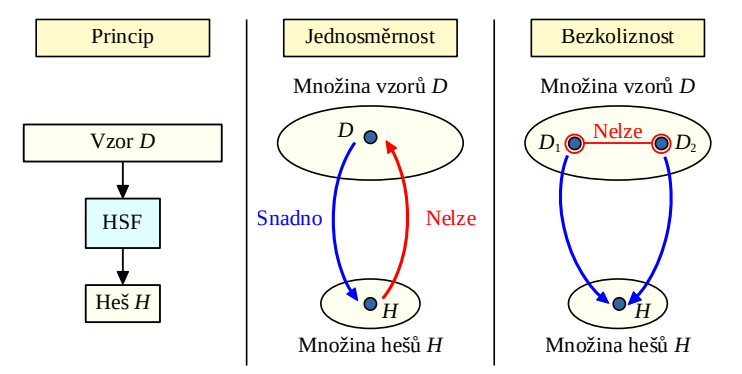
\includegraphics[width=0.8\textwidth, angle=0]{hesla-has.png}
 	\caption[Hesla hešovací funkce]{Hešovací funkce a její vlastnosti.}\label{fig:has}
\end{figure}
 
Kryprografické využití hešovacích funkcí:
 
\begin{itemize}
\item Kontrola integrity (kontrola shodnosti velkých souborů a dat).
\item Automatické dešifrování (souboru, disku apod.).
\item Ukládání a kontrola přihlašovacích hesel. 
\item Prokazování autorství.
\item Jednoznacná identifikace dat (jednoznačná reprezentace vzoru, digitální otisk dat, jednoznacný identifikátor dat, to vše zejména pro digitální podpisy).
\item Prokazování znalosti.
\item Autentizace původu dat.
\item Nepadělatelná kontrola integrity.
\item Pseudonáhodné generátory, derivace klíčů.
\end{itemize}

\subsubsection{MD5}
%http://crypto-world.info/klima/2005/cryptofest_2005.htm#_Toc98987082
%U MD5 tvoří kontext čtyři 32 bitová slova A, B, C a D. Na obrázku vidíme zvětšenu jednu rundu hašování. \( m_i \) je jeden 512 bitový blok zprávy. Ten je rozdělen na 16 32bitových slov \( M_0 M_1 \), \cdots, \( M_{15} \), a tato posloupnost je opakována 4x za sebou (v různých permutacích). 

%Na obrázku vidíme, že v kompresní funkci se kontext "zašifruje" vždy jedním 32bitovým slovem \( M_{i} \). Poznamenejme, že na místě dílčí funkce F v obrázku se po 16 rundách střídají 4 různé (nelineární i lineární) funkce (F, G, H, I) a v každé rundě se využívá jiná konstanta \( K_{i} \). Po 64 rundách dojde ještě k přičtení původního kontextu \( (H_i-1) \) k výsledku podle Davies-Meyerovy konstrukce (xor je nahrazen aritmetickým součtem modulo 232). Tak vznikne nový kontext \( H_{i} \). 

%Pokud by zpráva M měla jen jeden blok, byl by kontext (A, B, C, D) celkovým výsledkem. Pokud ne, pokračuje se stejným způsobem v hašování druhého bloku zprávy m_2 jakoby s inicializační hodnotou \( H_i-1 \). Po zpracování bloku \( m_N \) máme v registrech výslednou 128bitovou haš HN.

\begin{figure}[!ht]
	\centering
 	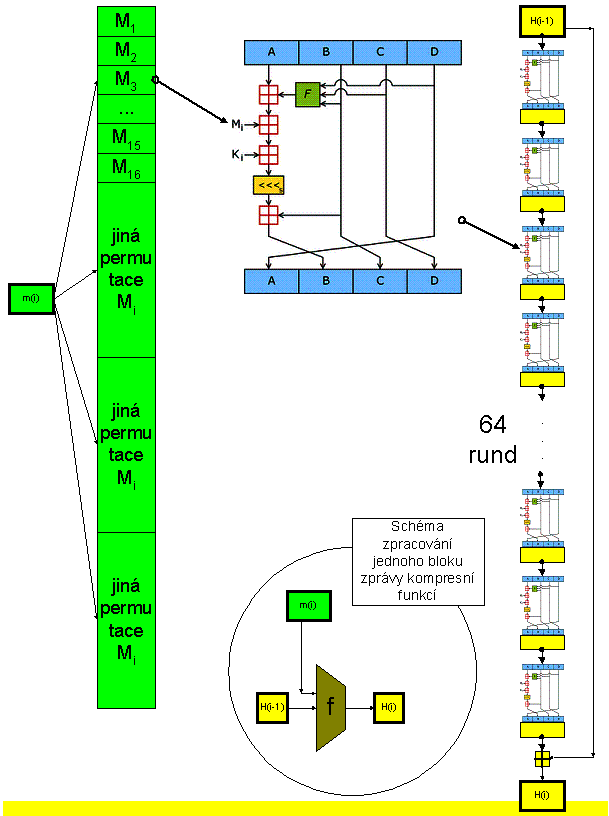
\includegraphics[width=0.8\textwidth, angle=0]{hesla-md5.png}
 	\caption[Hesla a hešovací funkce MD5]{Hešovací funkce MD5.}\label{fig:md5}
\end{figure}

\subsubsection{SHA-1}

Algoritmus SHA (Secure Hash Algorithm) byl zavedený NIST a publikovaný v norme FIPS 180 (1993). Revidovaná verze SHA–1 v normě FIPS–180–1 (1995). SHA–1 umožnuje zpracovat zprávu s %maximální délkou 2^64 − 1 bitů a představuje výstupní hašoví kód s délkou 160b. Vstupní
zpráva M je zpracována po blocích z velkosí 512b. Svým vnitřním fungováním je velice podobná MD5. Liší se zejména v velikosti výstupního řetězce. 

%Blok zprávy Mi
%je zpracováván v 4 × 20 rundách. 160 bitový
%kontext (opet za ˇ cínáme s inicializa ˇ cním vektorem ˇ IV ) je postupneˇ
%"zašifrováván"32b slovem mi pro rundy 0, 1, . . . , 15 a pro rundy
%16, 18, . . . , 79 32b slovem wi

Při inovaci standardu FIPS 180-1 na FIPS 180-2  byly zavedeny 3 nové hašovací algoritmy: SHA-256, SHA-384 a SHA-512. Jejich rozdíly je možné vidět v tabulce. 

%https://www.fit-wiki.cz/_media/%C5%A1kola/p%C5%99edm%C4%9Bty/bez-all.pdf

% parametry pro table: h! = nejblize
% p{5cm} na zalomovani bunky
\begin{table}[!ht]
  \begin{center}
	\caption{SHA-X vlastnosti}
    \label{tab:SHA-X}
    \begin{tabular}{|l|c|c|c|c|} 
    	  \hline
      \textbf{} & \textbf{SHA-1} & \textbf{SHA-256} & \textbf{SHA-384} & \textbf{SHA-512}\\
      \hline
	  Délka haš. kódu 		& 160  & 256  & 384   & 512\\
	  Délka zprávy 			& <264 & <264 & <2128 & <2128\\
	  Velikost bloku 		& 512  & 512  & 1024  & 1024\\
	  Velikost slova 		& 32   & 32   & 64    & 84\\
	  Počet rund 			& 80   & 80   & 80    & 80\\
	  Bezpecnost v bitech 	& 80   & 128  & 192   & 256\\
      \hline
    \end{tabular}
  \end{center}
\end{table}

\section{Útoky na hesla}
%https://www.csoonline.com/article/2130877/the-biggest-data-breaches-of-the-21st-century.html

Útoky na hesla jsou na denním pořádku na většinu z nás. Pokud se koukneme do blízké minulosti uvidíme, že firmy jako jsou např.: 

\begin{itemize}
	\item \textbf{Yahoo}, které v roce 2013 a 2014 unikly data milionů uživatelů. V roce 2013 to byl veliký problém, protože hesla nebyla pečlivě hešována. V roce 2014 se však již poučili a hesla zahešovali bcrypt algoritmem.
	\item \textbf{Marriott International}, útok se uskutečnil v roce 2014. Byl však objeven až v roce 2018. Během této doby bylo kompromitováno okolo 500 miliónů uživatelů. 
	\item \textbf{eBay}, roku 2014 unikly jména, adresy, data a hesla přes 145 miliónům uživatelů. Útok vyžadoval po zákazníkovi změnu hesla, ale přidal i kolonku na citlivé informace, které byly ukládány. 
	\item \textbf{Sony's PlayStation Network}, která byla napadena v roce 2011. Ztráty se odhadují na 171 miliónů dolarů. 12 miliónů kreditních karet, které byly uloženy bez jakého koliv zabezpečení bylo kompromitováno.
\end{itemize}

Jak lze vidět i v 21 století se hesla a další citlivé informace ukládají s velkou neopatrností a ledabilostí a to i u takových to známých firem. Seznam by mohl pokračovat do nekonečna, protože každým dnem útoků jen přibývá. 

Dále se podíváme na jedny z nejpoužívanějších praktik získávání a lámání hesel. V praktické části bude použit program Hashcat na provádění některých z níže uvedených útoků.

% https://www.onelogin.com/learn/6-types-password-attacks
\begin{itemize}
	\item \textbf{Slovníkový útok} využívá znalosti toho, že uživatelé tíhnou k používání hesel, jež jsou dobře známá slova. Pokud je politika použitého hesla přísnější, na začátku bude velké písmeno a na konci číslovka. Nemusí nad nimi poté těžce přemýšlet, jako nad náhodně vygenerovanými řetězci. Útočník potřebuje soubor, který obsahuje známá hesla. Takový není těžké najít kdekoliv na internetu. K testovaným útokům pomocí slovníku bude v pozdější části využit soubor rockyu.txt. 
	\item \textbf{Hrubá síla} již není tak efektivní, jako bývala před lety, kdy se začali používat a nutit po uživatelích hesla s alespoň 8 znaky. Tento útok je ve své podstatě nejjednodušší. Útočník spostí program, který mu generuje náhodné sekvence čísel a písmen ze sady, která byla použita při psaní hesla a zkouší veškeré možnosti. Jednoho dne se tedy určitě dostane na správnou posloupnost, ta se však s každým přidaným znakem exponenciálně vzdaluje.
	\item \textbf{Odposlech komunikace}. Útočník odposlechne komunikaci. Pokud je taková komunikace nešifrována je jednoduché z paketu získat heslo. Samoyřejmě to nemusí být pouze heslo, které se po síti přenáši. Proti takovým útokům se používá například SSL (Secure Sockets Layer) protkol, ten zajistí šifrování komunikace mezi subjekty.
	\item \textbf{Man In the Middle}, nebo-li MITM útok. Útočník se dostane do prostoru mezi uživatelem a např.: autentizačním serverem. Rozdíl mezi odposlechem je ten, že se rovnou napojí na linku a směruje provoz přes své zařízení. Takový útok je např. DNS sniffing.
	\item \textbf{Key logger attack}. Útočník nainstaluje software na hostitelský systém, který ukládá veškeré zmáčknutí klávesnice a následně data získá a analyzuje. Nemusí se však jednat pouze o SW, existují i USB rozbočovače, které se přípojí mezi klávesnici a USB port na systému.
	\item \textbf{Sociální inženýrství} je odvětví útoků, které cílý na neznalost uživatele, nebo jeho neopatrnost. Mezi takové patří: 
	\begin{enumerate}
		\item \textbf{Phishing}, se zaměřuje na kontaktování uživatele a donutí jej kliknout na závadný odkaz, či stáhnout např. kez logger skrze e-mail.
		\item \textbf{Baiting}, útočník nechá na chodníku kde se oběť pohybuje pohozené médium s útočným softwarem a počká až jej oběť sebere a dá jej do svého systému.
		\item \textbf{Quid quo pro}, kdy se útočník vydává za technockého zaměstnance a interaguje s obětí a donutí ji mu poskytnout cestu do systému.
	\end{enumerate}
\end{itemize}

%TODO table with attacks and protection

\section{Entropie hesla}




% https://vxempire.xyz/repo/Hash%20Crack.pdf

\subsection{Windows}

Windows se chovají jinak v doméně a jinak mimo ní. Pokud je počítač v doméně je preferován autentizační protokol kerberos. V současných Windows Server edicích je implementován Kerberos verze 5. Kerberos v základní nastavenim operuje na portu 88 a k šifrování používá symetrickou šifru. 
Pokud počítač není nastaven aby se autentikoval pomocí protokolu Kerberos používají Windows šifrování NTLM.

\subsection{Linux}

Hesla v linuxových systémech se skládají ze dvou konkretních souborů. 

/etc/shadow - obsah a strukturu toho souboru můžeme vidět na následujícím obrázku. 

% TODO Pictore of the structure  

/etc/passwd - obsah a strukturu tohoto souboru můžeme vidět na následujícím obrázku.

% TODO Pictore of the structure 

V /etc/shadow jsou hesla uložená pomocí hashe. 

\subsection{MacOS}

%TODO MacOS password handling

\section{Útoky na hesla}

\subsection{Hrubou silou}

\subsection{Pomocí masky}

\subsection{Se slovníkem}

\section{Entropie hesla}

\section{Ochrana před různými útoky}



% \input{realizace}

\chapter{Závěr}
\cite{merkel2014docker}1
	
% TODO get csns690
%\bibliographystyle{csn690}
\bibliographystyle{ieeetr}

\bibliography{mybibliographyfile}

\appendix

\chapter{Seznam použitých zkratek}
% \printglossaries
\begin{description}
	\item[GUI] Graphical user interface
	\item[XML] Extensible markup language
\end{description}



\chapter{Obsah přiloženého CD}

%upravte podle skutecnosti

\begin{figure}
	\dirtree{%
		.1 readme.txt\DTcomment{stručný popis obsahu CD}.
		.1 exe\DTcomment{adresář se spustitelnou formou implementace}.
		.1 src.
		.2 impl\DTcomment{zdrojové kódy implementace}.
		.2 thesis\DTcomment{zdrojová forma práce ve formátu \LaTeX{}}.
		.1 text\DTcomment{text práce}.
		.2 thesis.pdf\DTcomment{text práce ve formátu PDF}.
		.2 thesis.ps\DTcomment{text práce ve formátu PS}.
	}
\end{figure}

\end{document}

